\documentclass[addpoints,12pt]{exam}
\newcommand{\ds}{\displaystyle}
\usepackage[margin=0.8in]{geometry}
\usepackage{subcaption}
\usepackage{tikz}
\usepackage{amssymb,amsmath,graphicx,wrapfig,verbatim,wasysym, enumitem,psfragx,color}
\usepackage{multicol}


\usepackage{tikz}
\usepackage{graphicx,ctable,booktabs}

\usepackage{pgfplots}


\pgfplotsset{compat=1.10}
\usepgfplotslibrary{fillbetween}
\usetikzlibrary{patterns}
\pgfdeclarelayer{background}% determine background layer
\pgfsetlayers{background,main}% order of layers

%\usepackage{fancyhdr}
%\setlength{\headheight}{13.6pt}
%\pagestyle{fancy}
%\lhead{Math 222}
%\chead{ Midterm 1 }
%\rhead{Spring 2022}

\def\FillInBlank{\rule{3truein} {.01truein}}




% Choose one option (bubbles)
\newcommand{\chooseone}{{\Large$\Circle$\ \ }}
% Choose multiple options (squares)

\newcommand{\choosemany}{{\Large$\Square$\ \ }}


\newcommand{\myleft}{\makebox[.4\textwidth]{First Name:\enspace\hrulefill}}
\newcommand{\myright}{\makebox[.4\textwidth]{Last Name:\enspace\hrulefill}}
\header{\oddeven{\myleft}{}}
    {}
    {\oddeven{\myright}{}}

\footrule

\footer{Math 211}
     {Final Exam - Practice Exam}
     {Page \thepage\ of \numpages}

\begin{document}

\begin{questions}


\question Clearly mark the correct answer(s) for each of the following by completely filling in the
appropriate bubble. \textbf{No justification is needed.}

\begin{parts}


\part[2] \textbf{(Multiple Choice-Choose one)} The reproduction function for salmon in a fishery
is

$f(p)=-\frac{1}{10}p^2+13p$, where $p$ and $f(p)$ are in the thousands. The maximum
sustainable yield is which of the following?

\begin{itemize}[label={}]
\item \chooseone $60$ thousand
\item \chooseone $360$ thousand
\item \chooseone $420$ thousand
\item \chooseone None of the above.
\end{itemize}

\vfill

\part[2]\textbf{(Multiple Choice-Choose one)} If $f(x,y)$ has a critical point where $f_{xx}$ and
$f_{yy}$ are both positive, then...
\begin{itemize}[label={}]
\item \chooseone $f$ must have a relative minimum at that point.
\item \chooseone $f$ must have a relative maximum at that point.
\item \chooseone $f$ must have saddle point at that point.
\item \chooseone There is not enough information to classify the critical point.
\end{itemize}

\vfill




\part[2] \textbf{(True/False)} If $C(x,y)$ is the cost function for a soda factory for $x$ units of
Coca-Cola and $y$ units of Sprite, $C_x(x,y)$ is the marginal cost function for Sprite when the
production of Coca-Cola is held constant.

\begin{itemize}[label={}]
\item \chooseone True
\item \chooseone False
\end{itemize}

\vfill

\part[2] \textbf{(True/False)} $\ds\int_0^\infty \frac{1}{10000}dx$ converges.

\begin{itemize}[label={}]
\item \chooseone True
\item \chooseone False
\end{itemize}

\vfill


\part[2] \textbf{(Multiple Choice-Choose one)} Suppose a study indicates that the distribution of
income for lawyers is given by the Lorenz curve $L(x)=x^2$. Suppose the Gini index for doctors
is $0.5$. Which profession has the more equal distribution of income?

\begin{itemize}[label={}]
\item \chooseone Lawyers
\item \chooseone Doctors
\item \chooseone They are the same.
\end{itemize}

\vfill


\end{parts}

\newpage


\newpage


\newpage




\question The demand function $d(x)$ and supply function $s(x)$ for a particular commodity are
given as:
$$d(x)=131-\frac{1}{3}x^2, \; \; s(x)=50+\frac{2}{3}x^2$$
\begin{parts}
\part[4] Find the consumers' surplus at demand level $A=3$. You do not need to simplify your
final numerical answer.\vfill
\part[3] Find the market demand (the positive value of $x$ at which the demand function
intersects the supply function).\vfill
\part[4] Find the producers' surplus at market demand. You do not need to simplify your final
numerical answer.\vfill




\end{parts}


\newpage

\newpage
\question[8] Evaluate the following improper integral or show that it is divergent.

$\ds \int_0^\infty \dfrac{e^{2x}-e^{4x}}{e^{6x}}dx$


\newpage

\question
Calculate the derivative of each function. You do not need to simplify your answer.


\begin{parts}

\part[5] $f(x)=\dfrac{1}{x}+4\sqrt{x}-\sqrt{5}$


\vfill


\part[5] $\ds g(x)=\ln(3x-x^2)$


\vfill


\part[5] $F(x)=e^x(x^3+3x)$

\vfill

\part[5] $r(x)=\sqrt[3]{x^3+1}$

\vfill




\end{parts}

\newpage

%Revenue optimization

\question

Calculate each integral. You do not need to simplify your answer. Show all work.
\begin{parts}

\part[5] $\ds \int x^2(1-4x^3)dx $

\vspace{1.75in}

\part[5] $\ds \int \frac{1-\sqrt{x}}{\sqrt{x}} dx $

\vfill

\part[5] $\ds \int \left(\dfrac{3}{2x}+e^{-x}\right)dx $

\vfill

\end{parts}


\newpage




\question[8] The promoters of a state fair estimate that $t$ hours after the gates open at
9:00am, visitors will be entering the fair at the rate of $N'(t)=16-t^2$ hundred people per hour.
Find the total number of people who will enter the fair between 11:00am and 2:00pm. You do not
need to simplify the final numerical answer, but provide units.


\newpage

\question[8] Set up and evaluate the integral to compute the shaded area (see below) bounded
by the graphs $y=3-2x-x^2$ and $y=x-1$. You do not need to simplify your final numerical
answer.

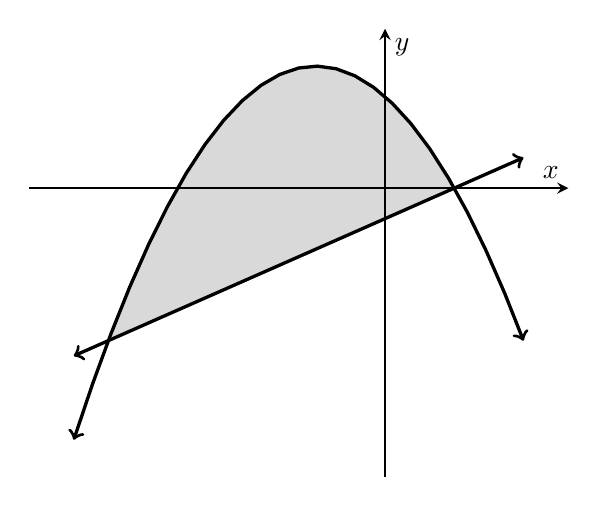
\begin{tikzpicture}[scale=1]
\begin{axis}[axis on top=true,axis lines=middle,axis line style = thick,
        xlabel=$x$,
        ylabel=$y$,
        enlargelimits,
        ytick=\empty,
        xtick=\empty
        ]

\addplot[name path=F,black, very thick,<->,domain={-4.5:2}] {x-1};

\addplot[name path=G,black,very thick,<->, domain={-4.5:2}] {3-2*x-x^2};


\addplot[color=gray!30]fill between[of=G and F, soft clip={domain=-4:1}];


%\node at (axis cs:2,2.45){};
\end{axis}
\end{tikzpicture}

\newpage




\newpage

\question For the function $f(x,y)=x^2+2y^2-x^2y$:
\begin{parts}
\part[5] Compute $f_{xx}, f_{yy},$ and $f_{xy}$. Show all work.
\vspace{3in}


\part[5] The critical points of $f(x,y)$ are $(0,0), (2,1)$, and $(-2,1)$. Determine, using the
$D$-test, if each point corresponds to a relative maximum, relative minimum, or saddle point.
Show all work.


\end{parts}
\vspace{0.25in}

\newpage


\question Given the following information about two functions, $g(x)$ and $f(x)$:
\begin{itemize}
       \item[] $f(3)=4$ \quad $f'(3)=-7$
       \item[] $g(3)=2$ \quad $g'(3)=5$
       \item[] $f(6)=8$ \quad $f'(6)=3$
\item[] $g(6)=9$\quad $g'(6)=10$

\end{itemize}
Compute each of the following. Simplify your answers.
\begin{parts}

      \part[2] $h'(3)$ if $h(x)=f(x)g(x)$.\vfill
      \part[2] $h'(6)$ if $h(x)=\dfrac{3f(x)}{4}$.\vfill
      \part[2] $\displaystyle \lim_{h\to 0}\dfrac{f(h+3)-f(3)}{h}$.\vfill
     \part[2] The average value of $g'(x)$ on $[3,6]$.\vfill
      \part[2] The relative rate of change of $g(x)$ at $x=3$.\vfill
\end{parts}




\newpage




\end{questions}

\end{document}
